\section{Model Description}
The radiation pressure module contains two different models for calculating the effects of solar radiation pressure on spacecraft state. Both methods of calculating solar radiation pressure have simple implementations in Basilisk using basic coefficients and assumptions. The methods of arriving at these coefficients can be complex and making the coefficients time-varying to improve accuracy can greatly increase complexity. The cannonball method used here essentially follows the mathematics described by Vallado\cite{vallado2001}.

\subsection{Radiation Pressure Model}
Radiation is modeled by using the solar flux at one astronomical unit and scaling by distance from the sun relative to 1 AU. The solar flux at one AU is taken as :
\begin{equation}
SF_{\mathrm{AU}} = 1372.5398    [W/m^2]
\end{equation}
\subsubsection{Cannonball Method}
The radiation pressure at 1AU, $p_{SR}$, can be taken as the solar flux divided by the speed of light. 
\begin{equation}
	p_{SR} = \frac{SF_{\mathrm{AU}}}{c}
\end{equation}
Then, a ``scaling factor'' can be determined. This ``scaling factor" is equivalent to the magnitude of the solar radiation force divided by the distance between the spacecraft and the sun:
\begin{equation}
	\frac{|\mathbf{F}_{\textrm{radiation}}|}{|\mathbf{r}_{\textrm{sun}}|} = \frac{-c_{R}p_{SR}A_{\odot}{AU}^2}{|\mathbf{r}_{\textrm{sun}}|^3}
\end{equation}
$\mathbf{r}_{\textrm{sun}}$ is the vector from the spacecraft to the sun in the spacecraft body frame. This factor is then multiplied by the position vector from the spacecraft to the sun to get the force on the spacecraft due to solar radiation pressure.
\begin{equation}
	{\mathbf{F}_{\textrm{radiation}}} = \frac{|\mathbf{F}_{\textrm{radiation}}|}{|\mathbf{r}_{\textrm{sun}}|}  \mathbf{r}_{\textrm{sun}}
\end{equation}
The user must provide the coefficient of reflection and the equivalent area of the spacecraft to use this method.\\
\subsubsection{Table Look-up Method}
For the table look-up method, pre-determined values of torque and force acting on the spacecraft due to radiation pressure are given. It is required that these values be given at 1AU from the sun and with a corresponding direction vector from the spacecraft to the sun in the spacecraft body frame.\\\\
The look-up works by finding the direction vector in the given tables which most closely matches the spacecraft's current position vector. This is done by taking the maximum of the dot products of each lookup vector entry with the sun heading vector in the body frame. As a visual demonstration, \ref{fig:lookupMethod} shows that for some current sun heading amongst the body vector entries 1 through 8, the force and torque data corresponding to entry 8 would be chosen due to its proximity to the current sun heading.
\begin{figure}[H]
	\centerline{
		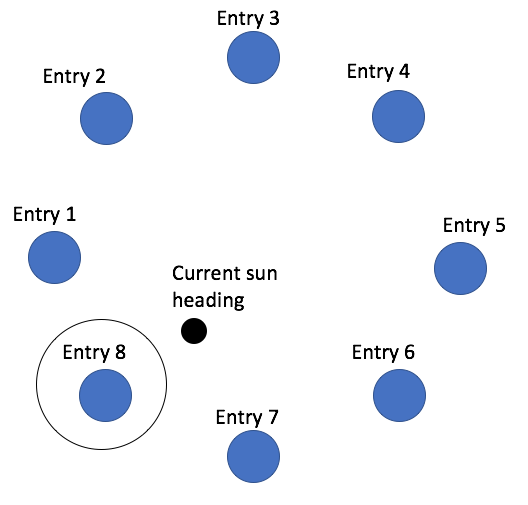
\includegraphics[height=0.5\textwidth, keepaspectratio]{Figures/lookupDiagram}}
	\caption{Visual Description of Table Look-up Method}
	\label{fig:lookupMethod}
\end{figure}


Then, the corresponding force and torque values are taken from the table and scaled according to the magnitude of the spacecraft-sun position vector:
\begin{equation}
{\mathbf{F}_{\textrm{radiation,scaled}}} = {\mathbf{F}_{\textrm{radiation}}}{\Big(  \frac{AU}{|\textbf{r}_{\textrm{sun}}|}  \Big)}^{2}
\end{equation}
\begin{equation}
{\mathbf{\tau}_{\textrm{radiation,scaled}}} = {\mathbf{\tau}_{\textrm{radiation}}}{\Big(  \frac{AU}{|\textbf{r}_{\textrm{sun}}|}  \Big)}^{2}
\end{equation}\\\\
Most important to the user of the table look-up method is the required input and format of data. Data must be recorded in XML format. As an example, see ../cube\_lookup.xml (in the radiation pressure folder). Additionally, a utility script called parseSRPLookup.py is provided there to read the XML input into numpy arrays. Experienced users are welcome to store their data in their own format and load it into equivalent numpy arrays as they see fit.\\\\
An example of using the provided python script to load data is shown in test\_radiationPressure.py. Note that this also requires import of the unitTestSupport library.\\
\subsubsection{Solar Eclipses}
Solar eclipses are are detected by the basilisk eclipse module. The effects of the eclipse are calculated into a shadow factor, $F_{\mathrm{s}}$, which is applied to the output forces and torques. 
\begin{equation}
\mathbf{F}_{\mathrm{out}} = F_{\mathrm{s}}\mathbf{F}_{\mathrm{full\_sun}}
\end{equation}
\begin{equation}
\bm{\tau}_{\mathrm{out}} = F_{\mathrm{s}}\bm{\tau}_{\mathrm{full\_sun}}
\end{equation}